\section*{Results}

% =====
% CRITICAL DENSITY
% =====

\subsection*{Critical density}

We characterize phase separation in terms of a ``critical system density'' at which the system separates into a sparse gas phase and dense clusters (based on a local density calculation detailed in the Methods section of the in-preparation paper).
We would expect that particle anisotropy should depress critical density relative to that seen in disks \cite{PrymidisEA_2016_SoftMatter}.
If we hypothesize that clustering follows the same mechanism as an equilibrium phase transition, we would expect the nature of this ``transition'' to mirror that of these shapes in equilibrium.
Specifically, work by Anderson \textit{et al.} suggested that shapes beyond 7-gons display a phase transition from fluid to hexatic to solid analogous to the transition seen in disks.
Naively, we might then expect that the critical density will decrease with decreasing $n$, and would expect phase separation behavior for $n{\geq}7$ to be indistinguishable from disks.

As shown in Figure \ref{fig:phase_diagram}A, we do observe a change in critical density relative to that seen in disks.
However, critical density does not correlate linearly with the number of particle sides, and is not uniformly depressed by the introduction of shape.
Instead, we see 6-gons phase separate at extremely low packing fractions (even at $\Phi=0.01$ in vertex-forward models). 
Next, 5-, 7-, and 8-gons phase separate at moderately low packing fractions.
Finally, 3- and 4-gons phase separate at similar or even higher critical densities than those of disks.

At first glance, this trend appears to correlate with (1) the free volume in the cluster and (2) the ability of the shape's densest packing to stabilize shear.
Particles in the cluster attempt to pack into their shape's densest packing \cite{AtkinsonEA_2012_PRE} (results not shown in Prelim Report).
For 6-gons, this results in a honeycomb lattice, while 5-, 7-, and 8-gons assemble into lattices with interstitial free space.
While 3- and 4-gons can completely tile space, their densest packings are not able to stabilize shear forces in the cluster. 
Unlike clusters of disks, which cannot sustain translational or rotational motion, clusters of shapes can maintain momentum.
This directional movement enables both stabilized grains and shear stresses between grains not seen in disks.
Consequently, clusters of 3- and 4-gon are fundamentally less stable than their higher-$n$ counter parts. 
This explanation also explains Prymidis \textit{et al}'s discovery of an ``oscillatory'' regime in their phase diagram \cite{PrymidisEA_2016_SoftMatter}.
We would expect to see such a regime in any shape whose densest packing is prone to shear planes.


\newpage
\vfill

\begin{figure*}[!ht]
\begin{center}
% width should be 17.8cm, cut to make room for caption until I can cut it down
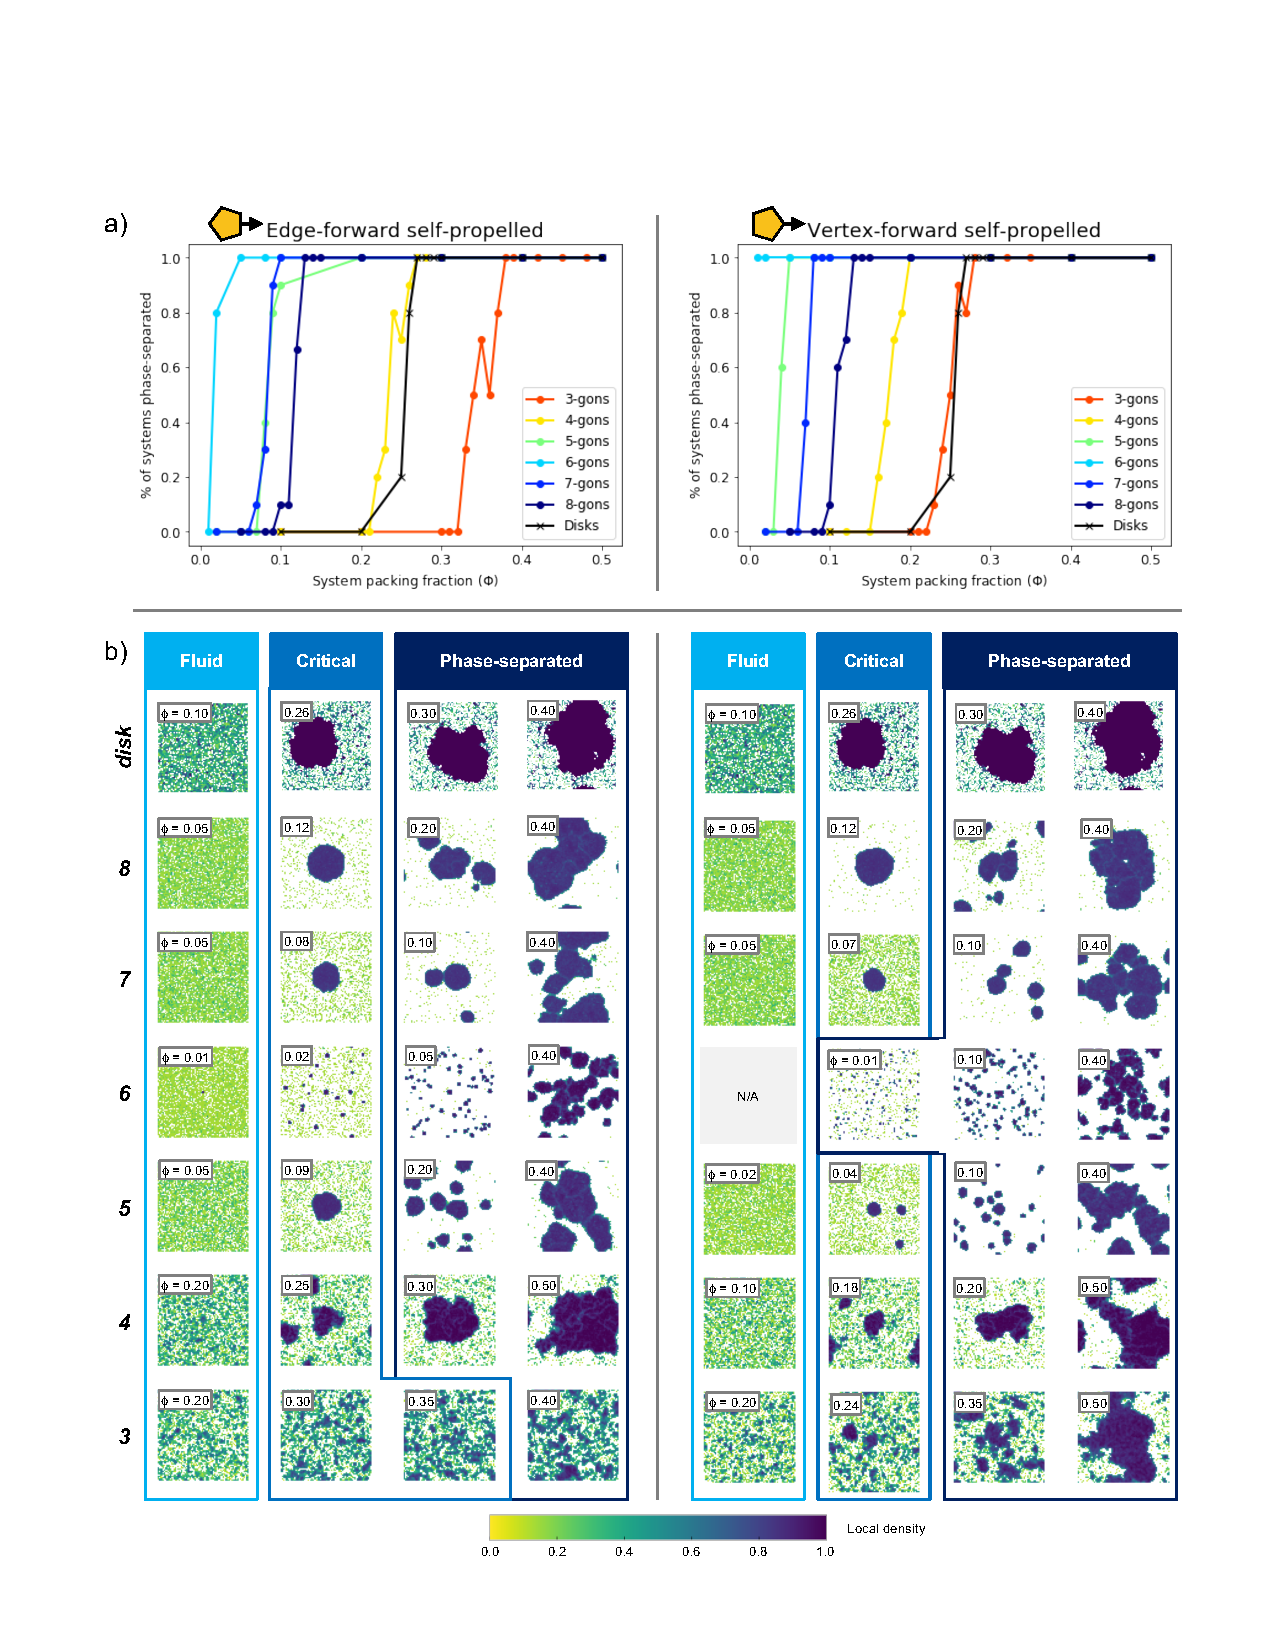
\includegraphics[width=6in]{../Figures/Fig2.pdf}
\caption{
\textbf{Critical density and nucleation behavior}:
(a) Ten replicates are studied at each $n$-gon and system packing fraction, and the fraction of replicates that phase-separate at steady state is determined as described in the Methods.
We see that the transition to phase separation is an abrupt one versus system packing fraction.
(b) Representative snapshots for the fluid (${\leq}0.10$ of systems phase separated), critical ($>0.1$ and $<0.9$), and phase-separated (${\geq}0.9$) regimes.
A distinctive feature of phase separation in systems of anisotropic particles is the formation of multiple stable clusters.
Large clusters at high packing fractions are formed by the collision of these multiple clusters.
%Grain boundaries resulting from these collisions can be seen in SI Figure \ref{sifig:structure}.
}
\label{fig:phase_diagram}
\end{center}
\end{figure*}

\vfill
\clearpage


% =====
% COLLECTIVE BEHAVIOR
% =====

\begin{figure*}[!t]
\begin{center}
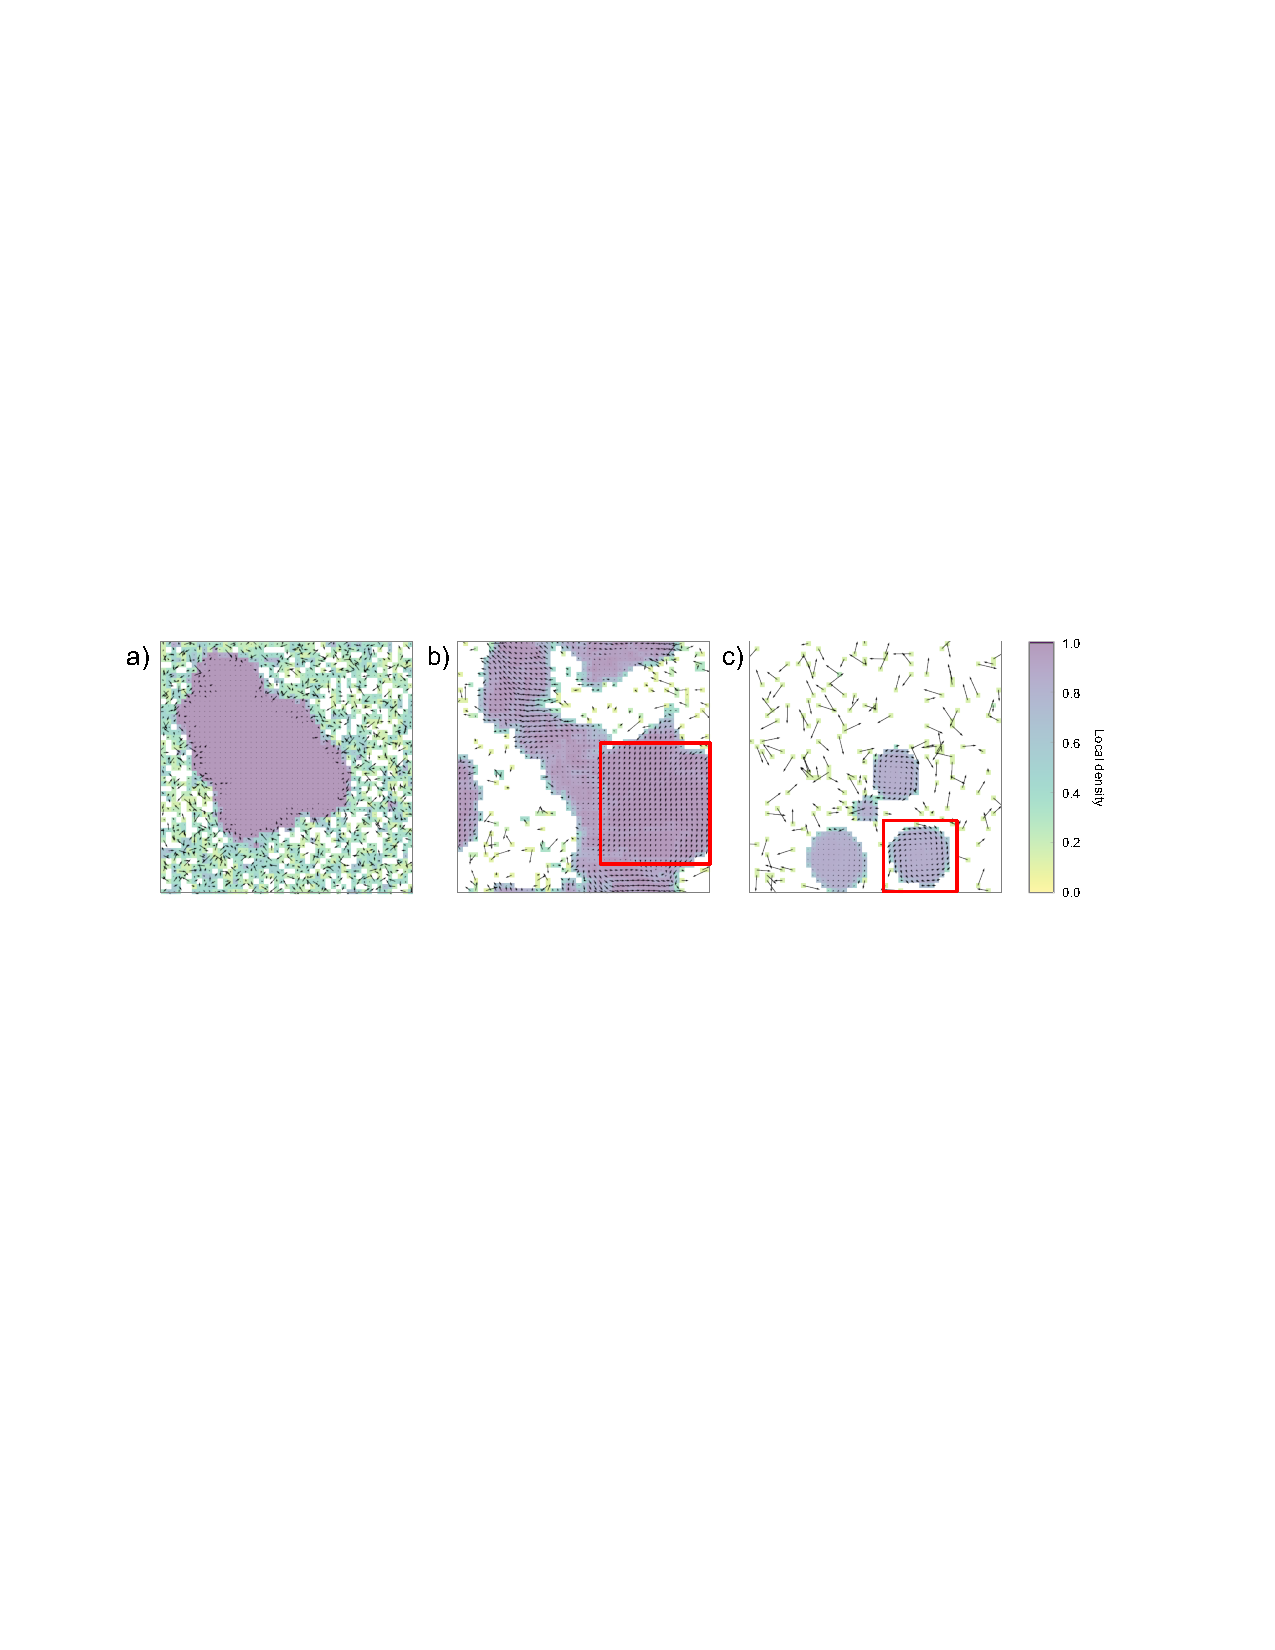
\includegraphics[width=6in]{../Figures/Fig4.pdf}
\caption{
\textbf{Cluster displacement}:
Shown are the particle displacement fields for simulations at steady state, laid over a map of local densities. 
(a) Clusters of disks have no net motion, with particle motion limited to the cluster boundaries and gas phase.
(Shown is a system of disks at $\Phi=0.3$).
In contrast, clusters with of shapes are able to convert particle translational forces to net motion (red insets).
Such clusters display both
(b) net translational motion (shown for $n=4$, $\Phi=0.5$, vertex-forward) and
(c) net rotational motion (shown for $n=7$, $\Phi=0.1$, edge-forward).
}
\label{fig:velocity}
\end{center}
\end{figure*}

\subsection*{Collective behavior}

Prior studies of driven shapes have observed that clusters are able to sustain rotational \cite{SumaEA_2014_EPL} and translational motion.
We also observe this behavior, as seen in Figure \ref{fig:velocity}.
As shown in Fig \ref{fig:velocity}A, clusters of disks do not have rotational or translational motion.
The only net motion within the cluster is at the boundaries, where a balance of particle fluxes in/out characterize the steady state configuration \cite{RednerEA_2013_PRL}.

However, to the best of our knowledge, other studies have not observed a key consequence of this ability: the formation of multiple small, stable clusters as precursors to bulk phase separation.
As seen in Fig. \ref{fig:phase_diagram}, phase separation in 5-, 7-, and 8-gons is characterized by the formation of one or few clusters which nucleate and grow.
In 6-gons, cluster nucleation is so favorable that we see the nucleation of many small clusters even in the critical regime.
For 3- and 4-gons, this picture is less clear but still points towards the formation of multiple small clusters as pre-cursors to phase separation.

In viewing videos of the evolutions of these systems (available during Preliminary Oral Exam), we see that at intermediate densities, these small clusters are stable.
This can also be seen in Figure \ref{fig:velocity}C, in which clusters are spinning in place.
At higher densities in systems of shapes, multiple small clusters form and translationally collide with one another to create larger clusters; evidence of these collisions can be seen in grain boundaries in large clusters at steady state.

In contrast, systems of isotropic particles cannot have multiple clusters collide, as clusters cannot sustain the motion required for a collision.
Instead, while multiple clusters may nucleate, a final system cluster is caused by either (1) smaller clusters dissolving and one large cluster dominating or (2) multiple smaller clusters merging into one another as they grow.
A steady state of multiple small clusters would be highly unlikely in a system of isotropic particles, as clusters in such systems are only stabilized by particles being self-propelled into the cluster.

This suggests that particle anisotropy allows these systems to pursue a different mechanism of nucleation.
Importantly, this mechanism of cluster formation does not appear to be achievable in disks. 
Redner \textit{et al.} investigated the addition of attraction to active isotropic particles at a constant packing fraction of $\Phi=0.4$ \cite{RednerEA_2013_PRE}.
At high activity and low attraction, that study replicated the formation of one large cluster seen in the literature.
At lower activities and high attraction, they were able to access a gel state; however, at no point in the activity/attraction phase space were multiple, clearly-separated stable clusters observed.  

% =====
% IMPACT OF SHAPE
% =====

\begin{figure*}[!t]
\begin{center}
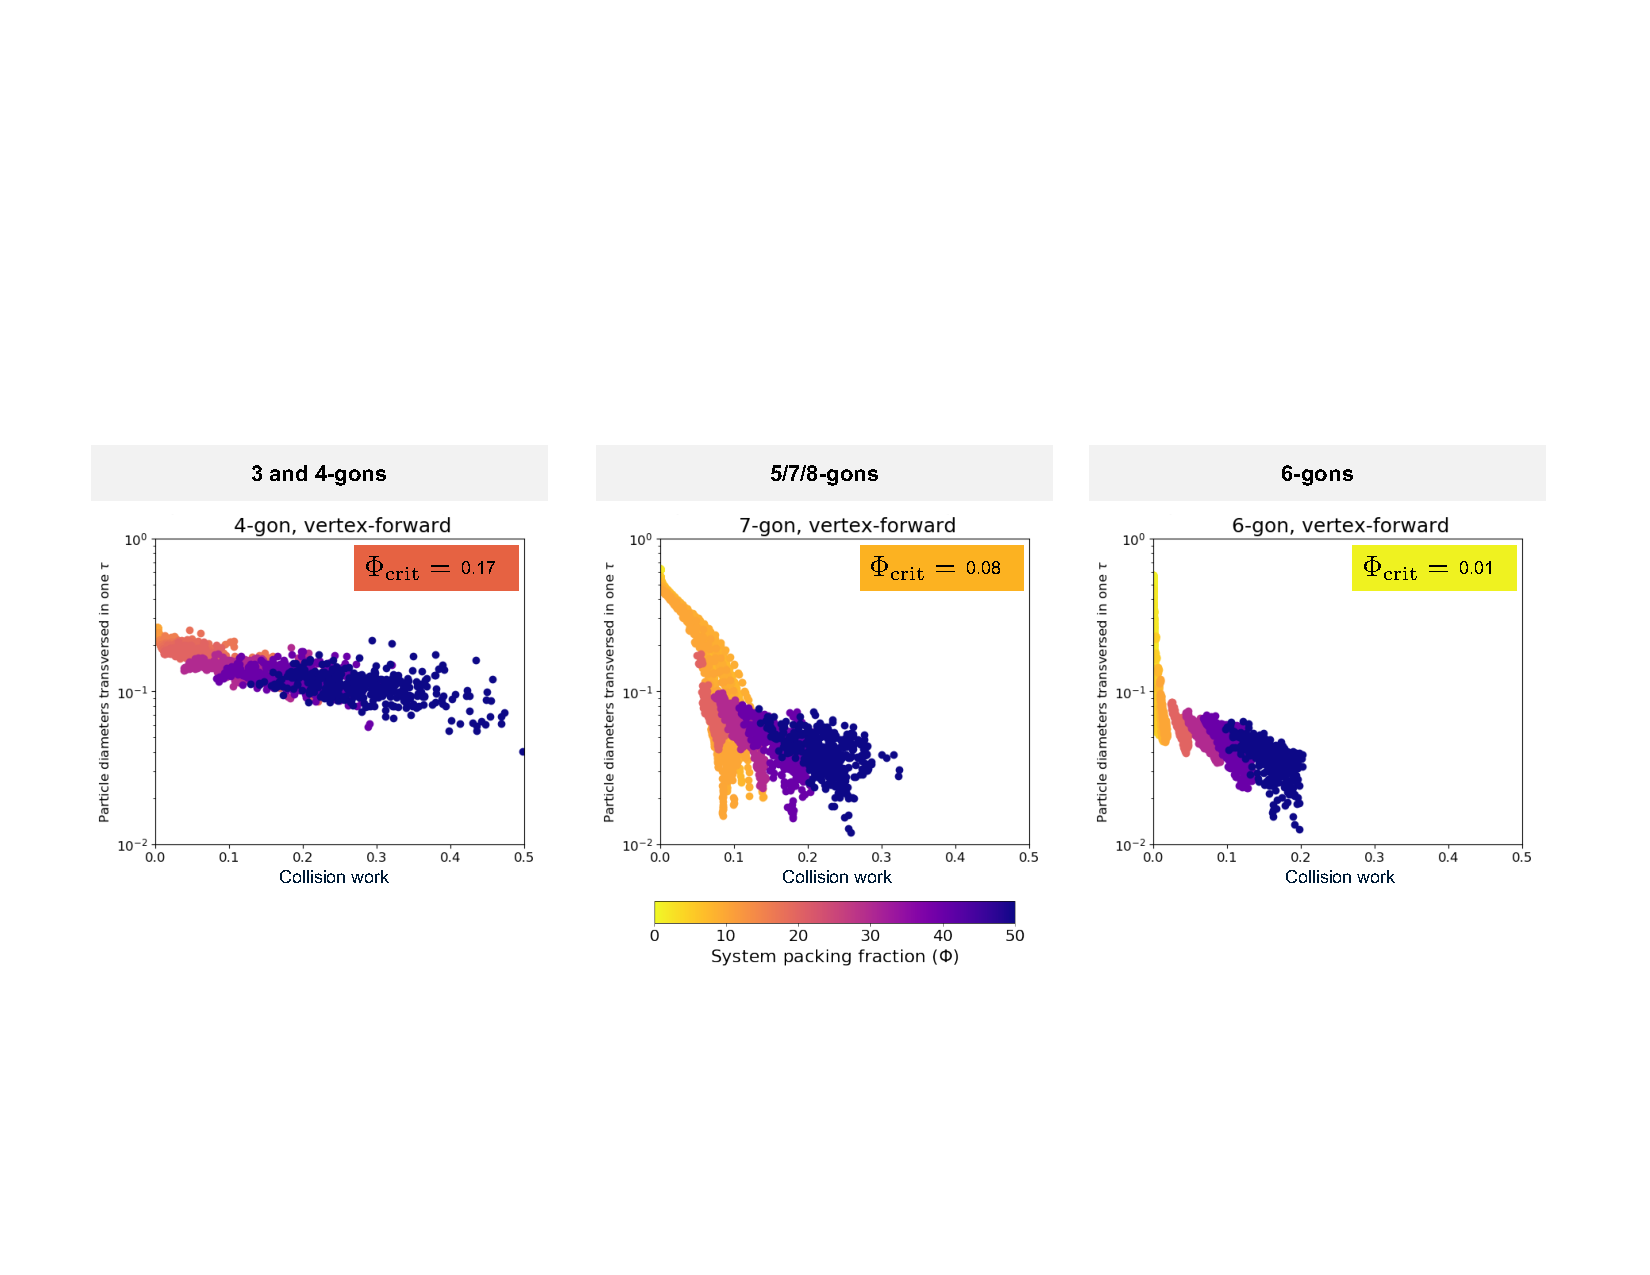
\includegraphics[width=6.5in]{../Figures/Fig3.pdf}
\caption{
\textbf{Collision efficiency}:
Shown are the evolution of particle velocity versus work done by inter-particle collisions in a system over the course of simulation.
Each system packing fraction is composed of ten replicates, with data snapshots taken approximately every $125\tau$.
Statepoints shown are representative of behavior in each group of $n$-gons.
}
\label{fig:pressure}
\end{center}
\end{figure*}

\subsection*{How anisotropy impacts the collective behavior}

While it is clear that shape and force anisotropy work together to impact the critical density and nucleation behavior, an explanation from existing theories is less clear. 
A kinetics-based theory developed in \cite{Redner_2016_PRL} treats cluster formation as a balance of in/out fluxes of particles at the boundary of a cluster.
This balance relies upon the assumption that particles can escape clusters when the direction of their active force diffuses above the horizon of the cluster (either solo or as part of a multi-particle escape event).
However, such diffusion is significantly stericly hindered in clusters of shapes.
While these assumptions work well in systems of disks where they correctly predict the formation of a large cluster which nucleates and grows in cases of phase separation, it is not clear how to tailor this theory to the behavior of systems of anisotropic particles. 

Alternatively, we can take a collision-theory based approach as described in \cite{Bruss_2017_arxiv}, which treats phase separation as the result when the average collision time ($\tau_C$) exceeds that of the average particle's free time between collisions ($\tau_F$).
Calculating the $\tau_F$ of the particles and assuming a constant $\tau_C$ for all shapes, we would expect to find 3-gons with the lowest critical density, with 8-gons the highest, not in line with our simulation results.
This confirms our intuition that the mechanism by which shapes depress the critical density is by increasing the collision time.

We posit that this increased collision time is the result of ``more effective'' collisions between some shapes versus others.
In the context of MIPS, we can  say that ``more effective'' collisions are those that translate inter-particle forces-- collisions-- to greater decreases in particle velocity.
That is, for a given collision, collisions between some particle shapes will lead to a steeper decreases in particle velocity than others.  
This also re-affirms our decision to study emergent behavior versus system density, a good proxy for the likelihood of inter-particle collisions that are required for phase separation to occur.

We can measure the net work done by all inter-particle collisions in the system as $ W = \frac{1}{2}\sum_i\sum_{j{\neq}i} \vec{F_{ij}}{\cdot}\vec{r_{ij}} $, where where $\vec{F_{ij}}$ and $\vec{r_{ij}}$ are the pairwise forces and distance between particles, respectively.
To study the efficiency of collisions for different shapes, we plot velocity versus the system's ``collision work'' in Figure \ref{fig:pressure}.
The velocity is shown as a percentage of the terminal velocity a particle would reach if it experienced no collisions.

We see that the evolution of velocity versus work done by collision follows very different patterns for the three groups of shapes.
Velocity quickly decreases with very little work for 6-gons, while velocities of 3 and 4-gon systems change little with collisions.
As might be expected from earlier results, 5/7/8-gons fall somewhere in between.

As presented, this data shows the time evolution for systems at each density, from start of the simulation (higher velocity) through steady state (lower velocity).
Next steps will be to probe the relaxation time from this data, which we expect to be shape-dependent given the obvious difference in velocity/work relationships in the critical regime for each group of shapes.
We are hopeful this will provide a definitive explanation for the role of shape in these systems.

%Enhanced collision time due to particle anisotropy allows such particles to phase separate at lower critical system densities than isotropic particles.
%We can borrow some concepts from percolation theory to think about this.
%Instead of the probability of a site being occupied, we have the probability of a collision (per some unit time) occurring at a given system density.
%The fraction of systems that phase-separated at a given system density, then, are analogous to the probability of there being a percolating cluster in a given sample


